\section{Schema E-R + business rules }
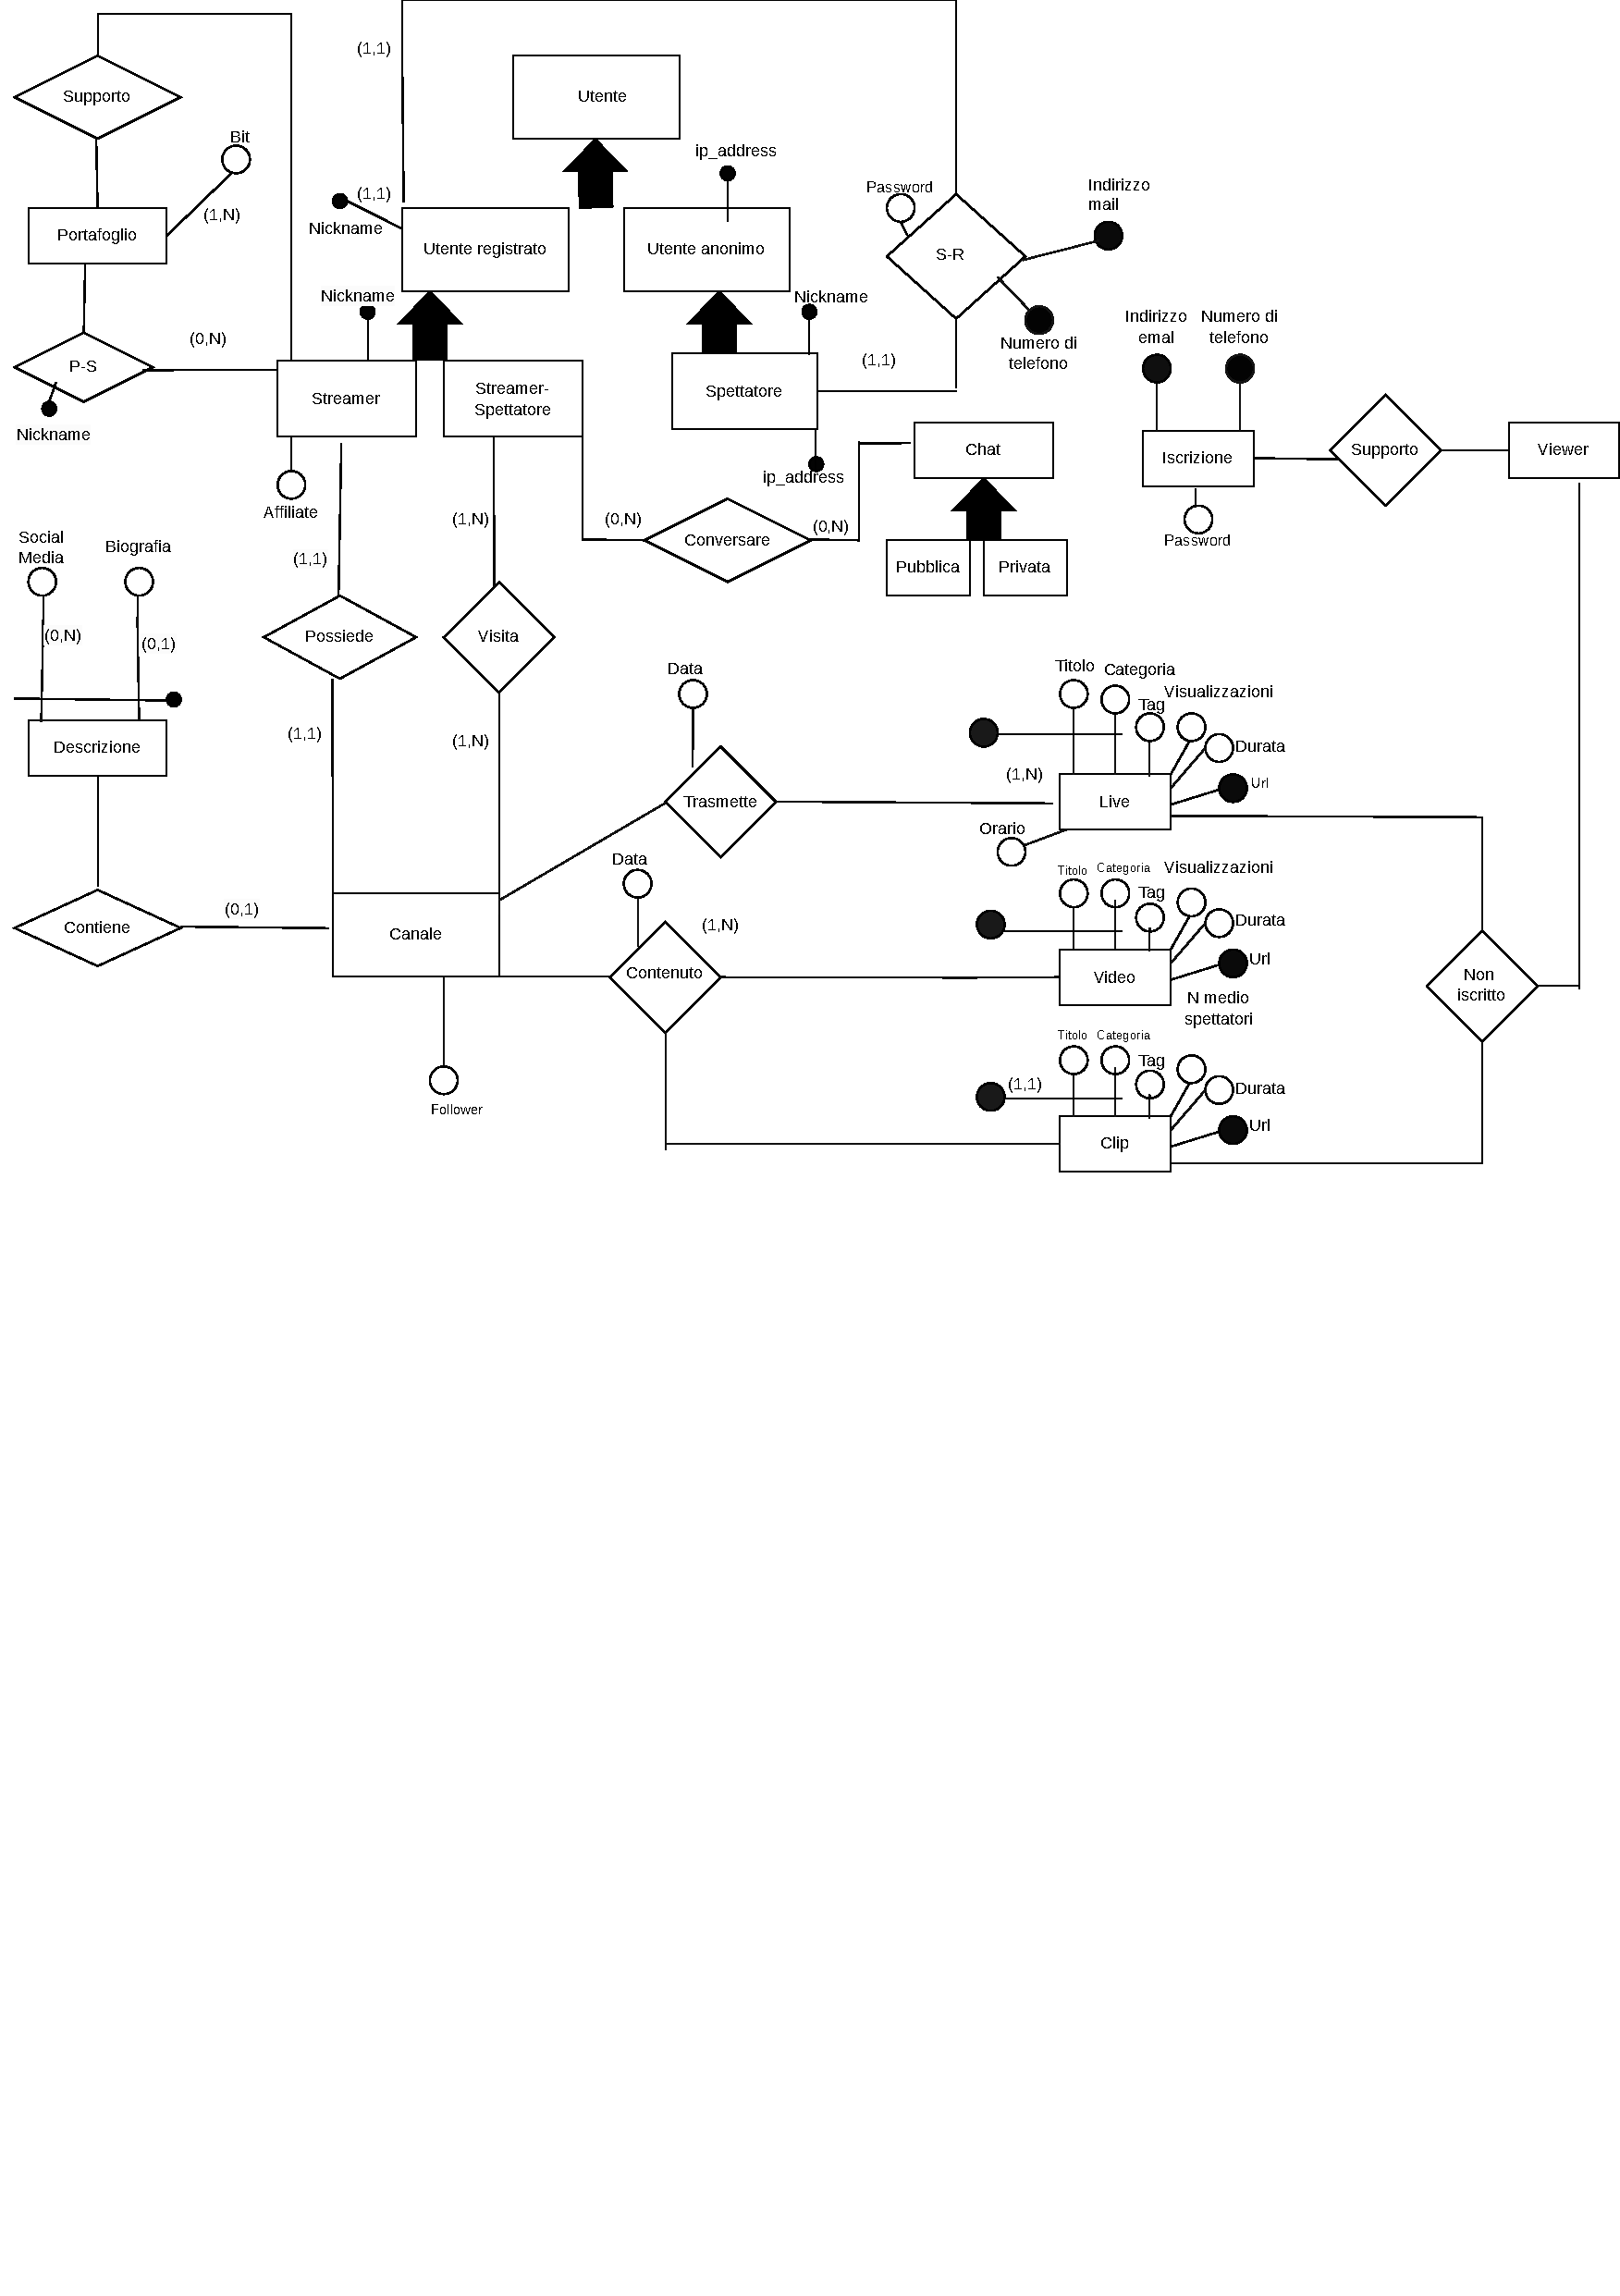
\includegraphics[width=\textwidth]{resources/schema_e-r.pdf}
\begin{itemize}
    \item I video sono degli estratti di live passate.
    \item Le clip sono dei video di breve durata.
    \item La moneta virtuale utilizzata è il bit, che può essere acquistato nella piattaforma.
    \item Un utente per registrarsi sulla piattaforma deve fornire indirizzo email o numero di telefono.
    \begin{itemize}
        \item Un utente anonimo può guardare la live trasmessa dallo streamer ma non può interagire con esso. 
    \end{itemize}
        \item Se uno \textit{streamer} rispetta i \textit{parametri di performance} può diventare \textit{affiliate}.
        \item Il portafoglio è costituito da \textit{bit}, con i quali il \textbf{follower}\footnote{solo il follower e non il viewer} può supportare lo streamer
        \item La chat permette agli utenti di comunicare l'uno con l'altro sia pubblicamente sia privatamente
\end{itemize}